\documentclass[aspectratio=169,11pt]{beamer}
\def\courseweek{2}
% Shared style for the Introduction to Information Geometry lecture slides.
% Compile the lecture .tex files from this directory.
\providecommand{\courseweek}{1}
\usepackage[T1]{fontenc}
\usepackage[utf8]{inputenc}
\usepackage[sc]{mathpazo}
\renewcommand{\sfdefault}{lmss}
\renewcommand{\ttdefault}{lmtt}
\usepackage{amsmath,amssymb,mathtools}
\usepackage{tikz}
\usetikzlibrary{arrows.meta,calc,positioning}
\usepackage{pgfplots}
\pgfplotsset{compat=1.18}
\usepackage{booktabs}

\definecolor{courseink}{HTML}{173749}
\definecolor{coursemuted}{HTML}{526674}
\definecolor{courseteal}{HTML}{0E7287}
\definecolor{coursecopper}{HTML}{B66B43}
\definecolor{courseline}{HTML}{D4E0E3}
\definecolor{coursepale}{HTML}{EFF5F5}

\setbeamercolor{normal text}{fg=courseink,bg=white}
\setbeamercolor{structure}{fg=courseteal}
\setbeamercolor{frametitle}{fg=courseink,bg=white}
\setbeamercolor{title}{fg=courseink}
\setbeamercolor{subtitle}{fg=coursemuted}
\setbeamercolor{block title}{fg=courseink,bg=white}
\setbeamercolor{block body}{fg=courseink,bg=white}
\setbeamercolor{alerted text}{fg=coursecopper}
\setbeamerfont{title}{family=\rmfamily,series=\bfseries,size=\fontsize{32}{37}}
\setbeamerfont{frametitle}{family=\rmfamily,series=\bfseries,size=\fontsize{26}{31}}
\setbeamerfont{normal text}{size=\fontsize{18}{22}}
\setbeamerfont{subtitle}{size=\fontsize{17}{21}}
\setbeamersize{text margin left=0.78cm,text margin right=0.78cm}
\setbeamertemplate{navigation symbols}{}
\setbeamertemplate{itemize items}[circle]
\setbeamertemplate{enumerate items}[default]
\setbeamertemplate{blocks}[default]
\setlength{\parskip}{0.22em}
\setbeamertemplate{footline}{%
  \leavevmode\hbox to \paperwidth{\hspace{.78cm}%
  {\color{coursemuted}\fontsize{8.5}{10}\selectfont Introduction to Information Geometry \hspace{.32cm} / \hspace{.32cm} Week \courseweek}%
  \hfill{\color{coursemuted}\fontsize{8.5}{10}\selectfont \insertframenumber\hspace{.17cm}/\hspace{.17cm}\inserttotalframenumber}\hspace{.78cm}}%
  \vskip.17cm
}
\setbeamertemplate{frametitle}{%
  \vspace{.13cm}
  \insertframetitle\par
  \vspace{.08cm}
}
\setbeamertemplate{title page}{%
  \vspace*{1.00cm}
  {\color{courseteal}\fontsize{10}{13}\selectfont\bfseries
  INTRODUCTION TO INFORMATION GEOMETRY\par}
  \vspace{.40cm}
  {\usebeamerfont{title}\usebeamercolor[fg]{title}\inserttitle\par}
  \vspace{.22cm}
  {\usebeamerfont{subtitle}\usebeamercolor[fg]{subtitle}\insertsubtitle\par}
  \vfill
  {\color{coursemuted}\fontsize{13}{16}\selectfont Christopher Lee\par}
  \vspace{.34cm}
}

\pgfplotsset{
  courseplot/.style={
    width=11.05cm,
    height=5.15cm,
    axis line style={coursemuted!75},
    tick style={coursemuted!65},
    ticklabel style={font=\scriptsize,color=coursemuted},
    label style={font=\normalsize,color=courseink},
    grid=major,
    major grid style={courseline!70,line width=.4pt},
    line width=1.45pt,
    legend style={font=\small,draw=none,fill=none,at={(.98,.03)},anchor=south east},
    clip=true
  }
}

\newcommand{\highlightmath}[1]{{\color{courseteal}#1}}
\newcommand{\thinrule}{\par\vspace{.25cm}{\color{courseline}\rule{\linewidth}{.8pt}}\par}

% A one-dimensional state space.  x=0 and x=1 are placed at 0 and 9 units.
\newcommand{\stateinterval}[1]{%
 \begin{tikzpicture}[x=1cm,y=1cm]
   \draw[courseink,line width=1.25pt] (0,0)--(9,0);
   \foreach \pos/\lab in {0/0,9/1} {
     \fill[courseink] (\pos,0) circle(2.7pt);
     \node[below=9pt,text=coursemuted] at (\pos,0) {\(\lab\)};
   }
   #1
 \end{tikzpicture}%
}

% Paired pages are separate frames in the PDF, with matching titles.
% Supply the whole frame body for each version; the instructor may edit them
% independently without changing overlay logic.
\newcommand{\coursepair}[3]{%
  \begin{frame}{#1}#2\end{frame}%
  \begin{frame}{#1}#3\end{frame}%
}

% Equilateral representation of the categorical simplex, in barycentric
% coordinates with vertices A=(0,0), B=(1,0), C=(1/2,sqrt(3)/2).
\newcommand{\coursesimplex}[1]{%
 \begin{tikzpicture}[scale=4.9]
  \fill[coursepale] (0,0)--(1,0)--(.5,.8660254)--cycle;
  \draw[courseink,line width=.65pt] (0,0)--(1,0)--(.5,.8660254)--cycle;
  \node[below left,font=\small] at (0,0) {A};
  \node[below right,font=\small] at (1,0) {B};
  \node[above,font=\small] at (.5,.8660254) {C};
  #1
 \end{tikzpicture}%
}

\title{Stability, Parameters, and Inference}
\subtitle{Week 2 \(\cdot\) Lecture 2}
\date{}
\begin{document}
\begin{frame}[plain]\titlepage\end{frame}

\begin{frame}{The derivative at an interior state}
Write \(\Delta(x)=\alpha+\beta x\), so
\[
F(x)=x(1-x)(\alpha+\beta x).
\]
\vspace{.37cm}
At an interior equilibrium \(x^*\), the factor \(\Delta(x^*)\) vanishes.
Differentiation gives
\vspace{.25cm}
\[
\highlightmath{F'(x^*)=\beta x^*(1-x^*)}.
\]
\vspace{.36cm}
The slope of the advantage line determines local attraction or repulsion.
\end{frame}

\coursepair{The local rate of coexistence}{
Take the familiar model
\[
F(x)=x(1-x)(3-4x),\qquad x^*=\tfrac34.
\]
\vspace{.44cm}
Find the linearization coefficient:
\[
F'(x^*)=\;?.
\]
\vspace{.32cm}
Is the equilibrium attracting or repelling?
}{
Take the familiar model
\[
F(x)=x(1-x)(3-4x),\qquad x^*=\tfrac34.
\]
\vspace{.44cm}
The advantage has slope \(\beta=-4\), so
\[
F'(x^*)=-4\cdot\frac34\cdot\frac14=\highlightmath{-\frac34}.
\]
\vspace{.32cm}
The equilibrium is attracting, with local decay \(u(t)\approx u(0)e^{-3t/4}\).
}

\begin{frame}{When linearization becomes inconclusive}
For \(F(x)=3x(1-x)^2\), the endpoint \(x=1\) attracts from the interior.
\vspace{.38cm}
\[
F'(1)=0.
\]
\vspace{.38cm}
Set \(u=1-x\). Near \(u=0\),
\[
u'=-3(1-u)u^2\approx-3u^2.
\]
\vspace{.35cm}
The displacement decays approximately like \(1/(3t+C)\).
The phase line settles the stability question.
\end{frame}

\begin{frame}{Changing one entry of a payoff matrix}
Consider the family
\[
M(a)=\begin{pmatrix}a&4\\3&1\end{pmatrix},\qquad
\Delta_a(x)=3+(a-6)x.
\]
\vspace{.40cm}
For \(a<3\), the interior equilibrium is
\[
\highlightmath{x^*(a)=\frac{3}{6-a}}.
\]
\vspace{.38cm}
It approaches \(x=1\) as \(a\) approaches \(3\) from below.
\end{frame}

\begin{frame}{A boundary bifurcation}
\vspace{-.22cm}
\begin{center}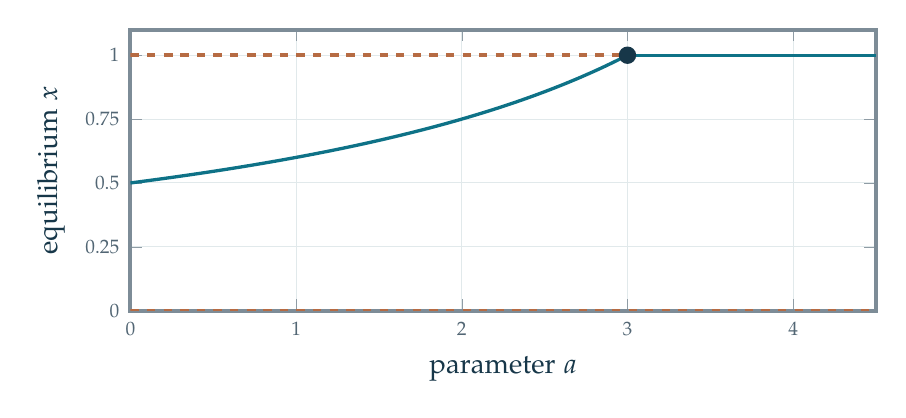
\begin{tikzpicture}
\begin{axis}[courseplot,xmin=0,xmax=4.5,ymin=0,ymax=1.10,
 xlabel={parameter $a$},ylabel={equilibrium $x$},xtick={0,1,2,3,4},
 ytick={0,.25,.5,.75,1}]
\addplot[courseteal,very thick,domain=0:3,samples=90]{3/(6-x)};
\addplot[courseteal,very thick,domain=3:4.5]{1};
\addplot[coursecopper,dashed,domain=0:3]{1};
\addplot[coursecopper,dashed,domain=0:4.5]{0};
\addplot[only marks,courseink,mark=*,mark size=2.4pt]coordinates{(3,1)};
\end{axis}\end{tikzpicture}\end{center}
\vspace{-.13cm}
At \(a=3\), the attracting interior branch meets the boundary.
\end{frame}

\begin{frame}{Payoff transformations}
Only the difference \(f_A-f_B\) enters the equation for \(x\).
\vspace{.40cm}
If \(\mathbf1=(1,1)^T\) and \(r=(r_A,r_B)^T\), then
\[
\highlightmath{\widetilde M=M+\mathbf1r^T}
\]
\vspace{.32cm}
adds the same opponent-dependent term \(r_Ax+r_B(1-x)\)
to both fitnesses.
\vspace{.36cm}
It changes their common growth level while preserving composition dynamics.
\end{frame}

\coursepair{Equivalent interaction matrices}{
Begin with \(M=\begin{pmatrix}2&4\\3&1\end{pmatrix}\).
Subtract the second row from both rows, column by column.
\vspace{.45cm}
\[
\widetilde M=\begin{pmatrix}?&?\\?&?\end{pmatrix}.
\]
\vspace{.35cm}
What is the resulting advantage \(\widetilde f_A-\widetilde f_B\)?
}{
Begin with \(M=\begin{pmatrix}2&4\\3&1\end{pmatrix}\).
Subtract the second row from both rows, column by column.
\vspace{.45cm}
\[
\highlightmath{\widetilde M=\begin{pmatrix}-1&3\\0&0\end{pmatrix}}.
\]
\vspace{.35cm}
Both matrices yield \(\widetilde f_A-\widetilde f_B=\highlightmath{3-4x}\).
}

\begin{frame}{Multiplying the payoffs}
If every payoff is multiplied by \(\lambda>0\), then
\[
\widetilde F(x)=\lambda F(x).
\]
\vspace{.53cm}
The same orbit is traversed at a different speed:
\[
\highlightmath{\widetilde x(t)=x(\lambda t)}.
\]
\vspace{.51cm}
The phase-line arrows and equilibrium positions stay the same.
\end{frame}

\coursepair{Designing a desired equilibrium}{
We want an attracting composition \(q=0.4\) with local rate \(u'=-0.6u\).
\vspace{.36cm}
Choose \(\Delta(x)=b(q-x)\).
\vspace{.35cm}
\[
F'(q)=-bq(1-q)=-0.6.
\]
\vspace{.35cm}
Find \(b\) and \(\Delta(x)\).
}{
We want an attracting composition \(q=0.4\) with local rate \(u'=-0.6u\).
\vspace{.36cm}
Choose \(\Delta(x)=b(q-x)\).
\vspace{.35cm}
\[
b=\frac{0.6}{(0.4)(0.6)}=\highlightmath{2.5}.
\]
\vspace{.35cm}
Then \(\highlightmath{\Delta(x)=1-2.5x}\).
}

\begin{frame}{A phase portrait constructed to order}
\vspace{-.20cm}
\begin{center}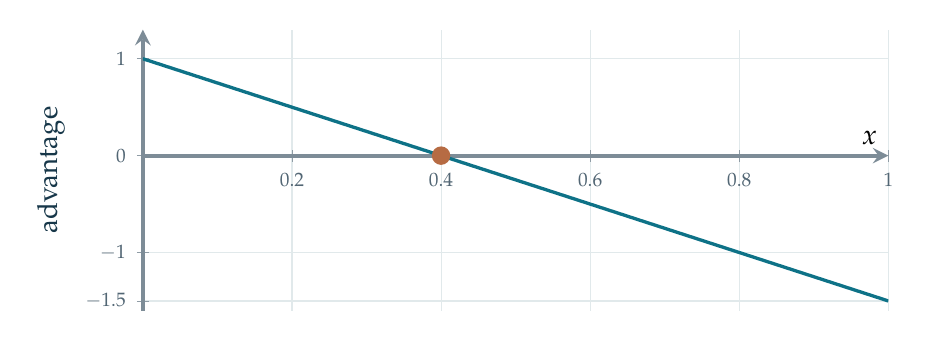
\begin{tikzpicture}
\begin{axis}[courseplot,xmin=0,xmax=1,ymin=-1.6,ymax=1.3,
 xlabel={$x$},ylabel={advantage},xtick={0,.2,.4,.6,.8,1},ytick={-1.5,-1,0,1},
 axis x line=middle,axis y line=left]
\addplot[courseteal,very thick,domain=0:1]{1-2.5*x};
\addplot[only marks,coursecopper,mark=*,mark size=2.6pt]coordinates{(.4,0)};
\end{axis}\end{tikzpicture}\end{center}
\vspace{-.12cm}
The zero specifies the target state. The slope controls its local return rate.
\end{frame}

\coursepair{Recovering an advantage from data}{
Measurements of instantaneous velocity give
\[
(x,x')=(0.2,0.16),\qquad(0.6,-0.24).
\]
\vspace{.28cm}
If \(\Delta(x)=\alpha+\beta x\), find \(\alpha\) and \(\beta\) using
\[
\Delta(x)=\frac{x'}{x(1-x)}.
\]
}{
Measurements of instantaneous velocity give
\[
(x,x')=(0.2,0.16),\qquad(0.6,-0.24).
\]
\vspace{.28cm}
The corresponding advantages are \(1\) and \(-1\).
Thus
\[
\highlightmath{\Delta(x)=2-5x},\qquad x^*=\frac25.
\]
}

\begin{frame}{Inference near a pure population}
The inferred advantage divides by \(x(1-x)\).
\vspace{.32cm}
\[
\Delta(x)=\frac{x'}{x(1-x)}.
\]
\vspace{.42cm}
A small error \(\varepsilon\) in the measured velocity changes the
advantage estimate by
\[
\highlightmath{\frac{\varepsilon}{x(1-x)}}.
\]
\vspace{.35cm}
For rare strategies, the same measurement error has a larger effect.
\end{frame}

\end{document}
